\documentclass[a4paper,14pt]{article}
\usepackage{float}
\usepackage{extsizes}
\usepackage{amsmath}
\usepackage{amssymb}
\everymath{\displaystyle}
\usepackage{geometry}
\usepackage{fancyhdr}
\usepackage{multicol}
\usepackage{graphicx}
\usepackage[brazil]{babel}
\usepackage[shortlabels]{enumitem}
\usepackage{cancel}
\usepackage{textcomp}
\usepackage{array} % Para melhor formatação de tabelas
\usepackage{longtable}
\usepackage{booktabs}  % Para linhas horizontais mais bonitas
\usepackage{float}   % Para usar o modificador [H]
\usepackage{caption} % Para usar legendas em tabelas
\usepackage{tcolorbox}
\usepackage{wrapfig} % Para usar tabelas e figuras flutuantes

\columnsep=2cm
\hoffset=0cm
\textwidth=8cm
\setlength{\columnseprule}{.1pt}
\setlength{\columnsep}{2cm}
\renewcommand{\headrulewidth}{0pt}
\geometry{top=1in, bottom=1in, left=0.7in, right=0.5in}

\pagestyle{fancy}
\fancyhf{}
\fancyfoot[C]{\thepage}

\begin{document}
	
	\noindent\textbf{6FMA56 - Matemática} 
	
	\begin{center}Adição e subtração com decimais (Versão estudante)
	\end{center}
	
	\noindent\textbf{Nome:} \underline{\hspace{10cm}}
	\noindent\textbf{Data:} \underline{\hspace{4cm}}
	
	%\section*{Questões de Matemática}
	\begin{multicols}{2}
    		\noindent Para somar ou subtrair números decimais, colocamos vírgula debaixo de vírgula e, se as quantidades de casas decimais forem diferentes, igualamos essas quantidades completando com zeros.\\
    		Exemplos: \\
    		\begin{itemize}
    			\item 3,23 + 1,59 = 4,82
    			\[
    			\begin{array}{ccc}
    				 & 3,23 \\
    				+ & 1,59 \\
    				\hline
    				& 4,82
    			\end{array}
    			\] \\
    			\item 4,7 + 2,2 = 2,5
    			\[
    			\begin{array}{ccc}
    				& 4,7 \\
    				- & 2,2 \\
    				\hline
    				& 2,5
    			\end{array}
    			\] \\
    			\item 9 + 0,12 + 6,7 = 15,82
    			\[
    			\begin{array}{ccc}
    				& ~ 9,00 \\
    				+ & ~ 0,12 \\
    				+ & ~ 6,70 \\
    				\hline
    				& 15,82
    			\end{array}
    			\] \\
    		\end{itemize}
    		\textsubscript{---------------------------------------------------------------------}
    		\begin{enumerate}
    			\item Calcule:
    			\begin{enumerate}[a)]
    				\item 1,7 + 0,6 \\\\\\\\\\\\
    				\item 3,1 + 7,4 + 2,6 \\\\\\\\\\\\
    				\item 1,8 + 5 + 0,4 \\\\\\\\\\\\
    				\item 8,7 - 3,4 \\\\\\\\\\\\
    				\item 6 - 0,3 \\\\\\\\\\
    				\item 15,2 - 8,9 \\\\\\\\\\\\
    			\end{enumerate}
    			\item Qual é a distância em km entre as cidades $A$ e $D$, ao longo de uma estrada reta, representada abaixo? \\
    			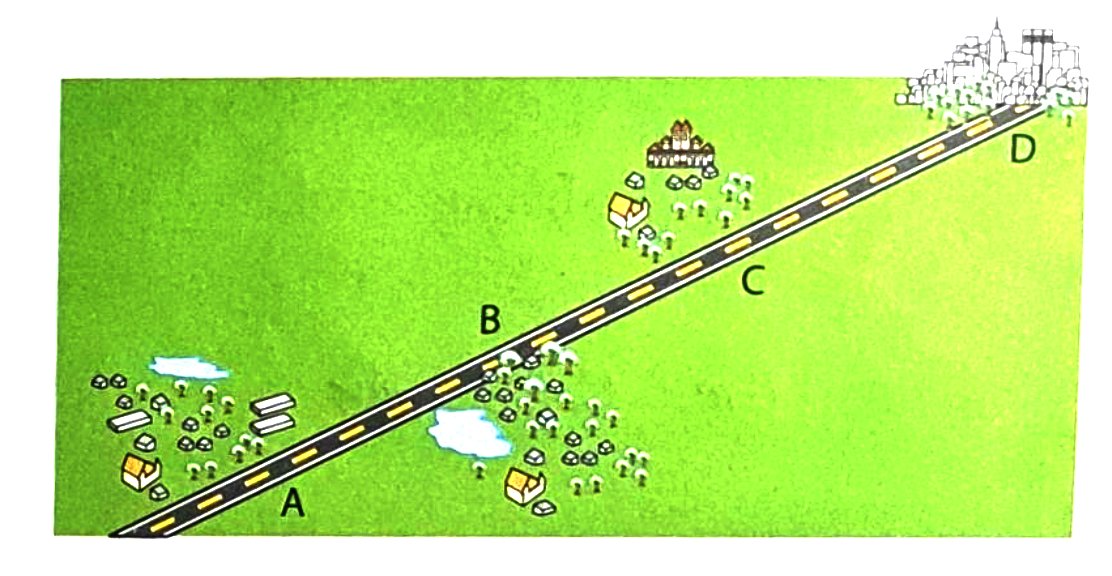
\includegraphics[width=1.1\linewidth]{6FMA56_imagens/imagem1}
    			\begin{itemize}
    				\item distância de $A$ até $C$: 105,2 km;
    				\item distância de $B$ até $D$: 76,45 km;
    				\item distância de $C$ até $B$: 30,7 km. \\\\\\\\\\\\\\\\
    			\end{itemize}
    			\item A distância entre duas prateleiras vizinhas está indicada na figura abaixo. Qual é a altura da estante?
    			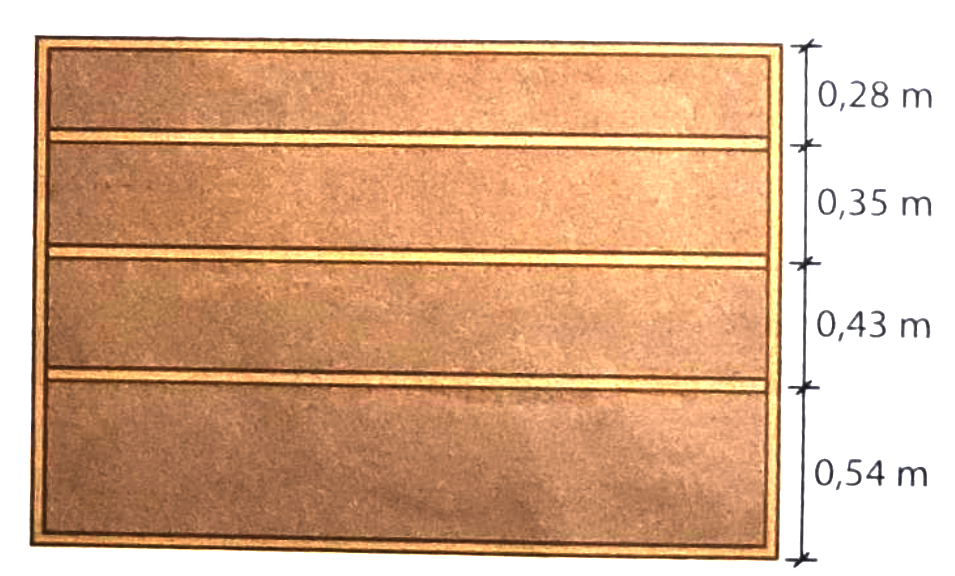
\includegraphics[width=1.1\linewidth]{6FMA56_imagens/imagem2} \\\\\\\\\\\\\\
    			\item Calcule:
    			\begin{enumerate}[a)]
    				\item 4,28 + 3,64 \\\\\\\\\\\\\\
    				\item 1,03 + 4,9 \\\\\\\\\\\\\\
    				\item 5,2 + 7,76 \\\\\\\\\\\\
    				\item 7,035 + 2,31 \\\\\\\\\\\\
    				\item 7,8 - 3,2 \\\\\\\\\\\\
    				\item 3,21 - 0,51 \\\\\\\\\\\\
    				\item 9,016 - 2,4 \\\\\\\\\\\\
    				\item 13,2 + 6,4 + 10,8 \\\\\\\\\\\\
    				\item 3,21 + 6,1 + 31,07 \\\\\\\\
    				\item 4,31 + 8,123 + 2,04 \\\\\\\\\\\\
    			\end{enumerate}
    			\item Considere o cardápio de uma lanchonete: \\\\
    			\begin{minipage}{0.45\textwidth} % Ajuste 0.45 para o tamanho adequado
    				\centering
    				\begin{tabular}{|c|c|}
    					\hline
    					\multicolumn{2}{|c|}{\textbf{Cardápio}} \\ % Linha mesclada
    					\hline
    					\textbf{Lanches} & \textbf{Preço} \\
    					\hline
    					cachorro-qte (simples) & R\$ 5,40 \\
    					\hline
    					cachorro-qte (completo) & R\$ 7,20 \\
    					\hline
    					\textbf{Bebidas} & \textbf{Preço} \\
    					\hline
    					suco natural & R\$ 8,10 \\
    					\hline
    					refrigerante (completo) & R\$ 6,30 \\
    					\hline
    				\end{tabular}
    			\end{minipage}
    			\\\\\\ Camila decidiu comer um cachorro-quente simples e tomar um refrigerante. Se ela comprar também um sorvete de 2,50 reais, quanto irá pagar? \newpage
    			\item (Enem) Em um parque há dois mirantes de alturas distintas que são acessados por elevador panorâmico. O topo do mirante 1 é acessado pelo elevador 1, enquanto que o topo do mirante 2 é acessado pelo elevador 2. Eles encontram-se a uma distância possível de ser percorrida a pé, e entre os mirantes há um teleférico que os liga que pode ou não ser utilizado pelo visitante.
    			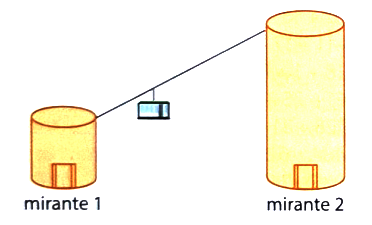
\includegraphics[width=1\linewidth]{6FMA56_imagens/imagem3} \\
    			O acesso aos elevadores tem os seguintes custos:
    			\noindent\begin{itemize}
    				\item Subir pelo elevador 1: \\ R\$ 0,15.
    				\item Subir pelo elevador 2: \\ R\$ 1,80.
    				\item Descer pelo elevador 1: \\ R\$ 0,10.
    				\item Descer pelo elevador 2: \\ R\$ 2,30. \\
    			\end{itemize}
    			O custo da passagem do teleférico partindo do topo do mirante 1 para o mirante 2 é de R\$ 2,00, e do topo do mirante 2 para o topo do mirante 1 é de R\$ 2,50. \\
    			Qual é o menor custo, em real, para uma pessoa visitar os topos do dois mirantes e retornar ao solo?
    			\begin{enumerate}[a)]
    				\item 2,25
    				\item 3,90
    				\item 4,35
    				\item 4,40
    				\item 4,45 \\\\
    			\end{enumerate}
    			\item Amanda foi a uma doceria e comprou uma barra de chocolate por 3,25, um pacote de balas por R\$ 8,36 e uma caixa de chicletes por R\$ 5,32. Quanto Amanda recebeu de troco se ela pagou com uma nota de R\$ 20,00? \\\\\\\\\\\\\\\\
    			\item Na figura abaixo, o segmento $\overline{BC}$ mede 98,40 mm, o segmento $\overline{CD}$ mede 23,42 cm e o segmento $\overline{AC}$ mede 12,71 cm. \\
    			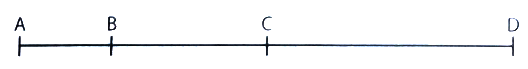
\includegraphics[width=1\linewidth]{6FMA56_imagens/imagem4} \\
    			Determine:
    			\begin{enumerate}[a)]
    				\item a medida de $\overline{AD}$. \\\\\\\\
    				\item a medida de $\overline{AB}$. 			
    			\end{enumerate}
    		\end{enumerate}
    		$~$ \\ $~$ \\ $~$
	\end{multicols}
\end{document}